
% This LaTeX was auto-generated from MATLAB code.
% To make changes, update the MATLAB code and republish this document.

\documentclass{article}
\usepackage{graphicx}
\usepackage{color}

\sloppy
\definecolor{lightgray}{gray}{0.5}
\setlength{\parindent}{0pt}

\begin{document}

    
    \begin{par}

\title{BE 521 - Homework 4\\{\normalsize Spring 2015}}
\author{Mike Lautman}
\date{\today}
\maketitle
\textbf{Objective:} Computational modeling of neurons.

\end{par} \vspace{1em}
\begin{verbatim}
close all; clear all; clc;
\end{verbatim}
\begin{par}

\section*{1 Simulating the Staba Detector}

\end{par} \vspace{1em}
\begin{par}

\subsection*{1.1 Number of Samples by Class}

\end{par} \vspace{1em}
\begin{verbatim}
dataset = 'I521_A0004_D001';
me = 'mlautman';
pass_file = 'mla_ieeglogin.bin';
[T, session] = evalc('IEEGSession(dataset, me, pass_file)');
data = session.data;
sample_rate = data.sampleRate ;
durration = data.channels(1).get_tsdetails.getDuration;
voltage_conv = data.channels(1).get_tsdetails.getVoltageConversion;
test_c = session.data.channels(1);
train_c = session.data.channels(2);
test = data.getvalues(1:test_c.getNrSamples,1);
train = data.getvalues(1:train_c.getNrSamples,2);
train_len_s = session.data.channels(2).get_tsdetails.getDuration;
test_len_s = session.data.channels(1).get_tsdetails.getDuration;

test_ann = data.annLayer(1);

train_ann = data.annLayer(2);

n_train_ev = train_ann.getNrEvents;

train_event = train_ann.getEvents(1,1);
train_events(n_train_ev) = train_event;
train_events(1) = train_event;
train_classes = zeros(1, n_train_ev);
train_classes(1) = train_event.description-48;

train_hfo_cnt = zeros(1,2);
train_hfo_cnt(train_classes(1)) = train_hfo_cnt(train_classes(1)) + 1;
for i=2:n_train_ev
    train_events(i) = train_ann.getNextEvents(train_events(i-1),1);
    train_classes(i) = train_events(i).description-48;
end

n_test_ev = test_ann.getNrEvents;

test_event = test_ann.getEvents(1,1);
test_events(n_test_ev) = test_event;
test_events(1) = test_event;
test_classes = zeros(1, n_test_ev);
test_classes(1) = test_event.description-48;

test_hfo_cnt = zeros(1,2);
test_hfo_cnt(test_classes(1)) = test_hfo_cnt(test_classes(1)) + 1;
for i=2:n_test_ev
    test_events(i) = test_ann.getNextEvents(test_events(i-1),1);
    test_classes(i) = test_events(i).description-48;
end


hfos= find(train_classes==2);
artifacts = find(train_classes==1);

number_of_hfos = length(hfos)
number_of_artifacts = length(artifacts)
\end{verbatim}

        \color{lightgray} \begin{verbatim}
number_of_hfos =

   101


number_of_artifacts =

    99

\end{verbatim} \color{black}
    \begin{par}

\subsection*{1.2 Plot 1 HFO and 1 Artifact}

\end{par} \vspace{1em}
\begin{verbatim}
figure(1)

subplot(1,2,1)
a1 = train_events(artifacts(1));
s = ceil(a1.start/train_len_s*length(train));
e = ceil(a1.stop/train_len_s*length(train));
vals = train(s:e);
time = (1:length(vals))/sample_rate;
plot(time, vals)
title('First tagged Artifact')
xlabel('Time (S)')
ylabel('Voltage (V)')
xlim([0,max(time)])
set(gca,'YTick',[])

subplot(1,2,2)
hfo1 = train_events(hfos(1));

s = ceil(hfo1.start/train_len_s*length(train));
e = ceil(hfo1.stop/train_len_s*length(train));
vals = train(s:e);
time = (1:length(vals))/sample_rate;
plot(time, vals)
title('First tagged HFO')
xlabel('Time (S)')
ylabel('Voltage (V)')
xlim([0,max(time)])
set(gca,'YTick',[])
\end{verbatim}

\includegraphics [width=4in]{mlautman_hw4_01.eps}
\begin{par}

\subsection*{1.3 FIR}

\end{par} \vspace{1em}
\begin{par}

\subsection*{1.4 Plot 1 HFO and 1 Artifact with FIR}

\end{par} \vspace{1em}
\begin{verbatim}
%
% Fs = sample_rate;  % Sampling Frequency
% N      = 100;   % Order
% Fstop1 = 10;    % First Stopband Frequency
% Fpass1 = 60;    % First Passband Frequency
% Fpass2 = 500;   % Second Passband Frequency
% Fstop2 = 600;   % Second Stopband Frequency
% Wstop1 = 1;     % First Stopband Weight
% Wpass  = 1;     % Passband Weight
% Wstop2 = 1;  % Second Stopband Weight
% dens   = 100;   % Density Factor
%
% filter = firpm(N, [0 Fstop1 Fpass1 Fpass2 Fstop2 Fs/2]/(Fs/2), [0 0 1 1 0 0], [Wstop1 Wpass Wstop2], {dens})*3.45e2;
load('Coefficients.mat');
figure(2)

subplot(1,2,1)
hold on

a1 = train_events(artifacts(1));

s = ceil(a1.start/train_len_s*length(train));
e = ceil(a1.stop/train_len_s*length(train));

vals = train(s:e);
time = (1:length(vals))/sample_rate;
plot(time, vals, 'b')
vals = filtfilt(Num,1,vals);
plot(time, vals, 'r')
title('First tagged Artifact with bandpass filter')
xlabel('Time (S)')
ylabel('Voltage (V)')
xlim([0,max(time)])
set(gca,'YTick',[])
legend('Raw', 'Filtered')

subplot(1,2,2)
hold on
hfo1 = train_events(hfos(1));

s = ceil(hfo1.start/train_len_s*length(train));
e = ceil(hfo1.stop/train_len_s*length(train));

vals = train(s:e);
time = (1:length(vals))/sample_rate;
plot(time, vals, 'b')
vals = filtfilt(Num,1,vals);
plot(time, vals, 'r')
title('First tagged HFO with bandpass filter')
xlabel('Time (S)')
ylabel('Voltage (V)')
xlim([0,max(time)])
set(gca,'YTick',[])
legend('Raw', 'Filtered')
\end{verbatim}

\includegraphics [width=4in]{mlautman_hw4_02.eps}
\begin{par}

\subsection*{1.5 Issues with Staba's Method}
Detecting HFO's poses a complex problem for automated systems. The
data we have been presented is extreemely noisy which makes tagging HFO's
very difficult. By normalizing the HFO and artifact recordings to zero
mean and unit standard deviation, the method increases the noise on low
amplitude signals causing them to become nearly indistinguishable from
HFOs.

\end{par} \vspace{1em}
\begin{par}

\section*{2 Defining Features for HFOs}

\end{par} \vspace{1em}
\begin{par}

\subsection*{2.1 }

\end{par} \vspace{1em}
\begin{verbatim}
trainFeats = zeros(n_train_ev,2);
testFeats = zeros(n_test_ev,2);

line_length = @(x) sum(abs(diff(x)));
area = @(x) sum(abs(x));

figure(3)
hold on

for i=1:n_train_ev

    s = max(ceil(train_events(i).start/train_len_s*length(train)),1);
    e = min(ceil(train_events(i).stop/train_len_s*length(train)),length(train));


    trainFeats(i,1)=line_length(train(s:e));
    trainFeats(i,2)=area(train(s:e));

    if train_events(i).description == '1'
        scatter(trainFeats(i,1), trainFeats(i,2), 'r')
    else
        scatter(trainFeats(i,1), trainFeats(i,2), 'b')
    end

end
legend('HFO', 'Artifact')



for i=1:n_test_ev

    s = max(ceil(test_events(i).start/test_len_s*length(test)),1);
    e = min(ceil(test_events(i).stop/test_len_s*length(test)),length(test));
    testFeats(i,1)=line_length(test(s:e));
    testFeats(i,2)=area(test(s:e));

%     if test_events(i).description == '1'
%         scatter(testFeats(i,1), testFeats(i,2), 'k')
%     else
%         scatter(testFeats(i,1), testFeats(i,2), 'g')
%     end
end

title('Line Length vs Area for HFO and artifacts')
xlabel('Line Length')
ylabel('Area')
\end{verbatim}

\includegraphics [width=4in]{mlautman_hw4_03.eps}
\begin{par}

\subsection*{2.2 Normalization}

\end{par} \vspace{1em}
\begin{verbatim}
mean_train = mean(trainFeats,1);
std_train = std(trainFeats,1);

trainFeats = bsxfun(@minus, trainFeats, mean_train);
trainFeats = bsxfun(@rdivide, trainFeats, std_train);

testFeats = bsxfun(@minus, testFeats, mean_train);
testFeats = bsxfun(@rdivide, testFeats, std_train);
\end{verbatim}
\begin{par}

\subsection*{2.2a Normalization}
mean and standard deviation

\end{par} \vspace{1em}
\begin{par}

\subsection*{2.2b Normalization for K-NN}
Normalization is essential in computing the distance metric for k-NN.
Without normalizing, if a single feature had a standard deviation of 3
times another feature, the second feature would have disproportionately
less influence on the distance calculation.

\end{par} \vspace{1em}
\begin{par}

\subsection*{2.2c Why use the training data mean and std?}
When normalizing the test data we use the mean and standard deviation
from the training data. In general, the test not available at the time
the model is being built so we use the training data when building the
preprocessing tranformations to simulate this.

\end{par} \vspace{1em}
\begin{par}

\section*{3 Comparing Classifiers}

\end{par} \vspace{1em}
\begin{par}

\subsection*{3.1 Training Error}

\end{par} \vspace{1em}
\begin{verbatim}
log_reg = mnrfit(trainFeats, train_classes);

train_pred_prob = mnrval(log_reg, trainFeats);
[~,Y_train_pred] = max(train_pred_prob,[],2);
train_error_percent = sum(Y_train_pred' ~= train_classes)/length(train_classes)
\end{verbatim}

        \color{lightgray} \begin{verbatim}
train_error_percent =

    0.1250

\end{verbatim} \color{black}
    \begin{par}

\subsection*{3.1 Test Error}

\end{par} \vspace{1em}
\begin{verbatim}
test_pred_prob = mnrval(log_reg, testFeats);
[~,Y_test_pred] = max(test_pred_prob,[],2);
test_error_percent = sum(Y_test_pred' ~= test_classes)/length(test_classes)
\end{verbatim}

        \color{lightgray} \begin{verbatim}
test_error_percent =

    0.1357

\end{verbatim} \color{black}
    \begin{par}

\subsection*{3.2 Test Error > Train Error}
It is reasonable for the Test error to be greater thant the training
error because the model was optimized to minimize misclassification
errors on the training data and not the test data. In that way, the test
data error gives us an idea of how well the learning algorithm
generalizes to unseen data.

\end{par} \vspace{1em}
\begin{par}

\subsection*{3.3a K-NN testing error}

\end{par} \vspace{1em}
\begin{verbatim}
knn_pred_test = knnclassify(testFeats,trainFeats, train_classes);
knn_pred_train = knnclassify(trainFeats,trainFeats, train_classes);

knn_test_error = sum(knn_pred_test' ~= test_classes)/length(test_classes)
knn_train_error = sum(knn_pred_train' ~= train_classes)/length(train_classes)
\end{verbatim}

        \color{lightgray} \begin{verbatim}
knn_test_error =

    0.1738


knn_train_error =

     0

\end{verbatim} \color{black}
    \begin{par}

\subsection*{3.4 SVM defaults}

\end{par} \vspace{1em}
\begin{verbatim}
train_classesT = train_classes';
test_classesT = test_classes';

svm_model = svmtrain(train_classesT, trainFeats);

[T, test_svm_pred_class, test_acc_svm, ~] = ...
    evalc('svmpredict(test_classesT, testFeats, svm_model)');
[T, train_svm_pred_class, train_acc_svm, ~] = ...
    evalc('svmpredict(train_classesT, trainFeats, svm_model)');

test_err_svm = sum(test_svm_pred_class' ~= test_classes)/length(test_classes)
train_err_svm = sum(train_svm_pred_class' ~= train_classes)/length(train_classes)
\end{verbatim}

        \color{lightgray} \begin{verbatim}
test_err_svm =

    0.1119


train_err_svm =

    0.1150

\end{verbatim} \color{black}
    \begin{par}

\subsection*{3.5 Decision Boundary}

\end{par} \vspace{1em}
\begin{verbatim}
training_1 = trainFeats(train_classes==1, :);
training_2 = trainFeats(train_classes~=1, :);

[X,Y] = meshgrid(-2:.01:3, -3:.01:5);
[n,d] = size(X);
X = reshape(X, [n*d,1]);
Y = reshape(Y, [n*d,1]);
F = [X,Y];
XC = ones(length(X),1);

figure(4)

[T, pred_class, ~, ~] = ...
    evalc('svmpredict(XC, F, svm_model)');

hold on
Xy = X(find(pred_class==1));
Xc = X(find(pred_class~=1));
Yy = Y(find(pred_class==1));
Yc = Y(find(pred_class~=1));
scatter(Xy, Yy, '.', 'y')
scatter(Xc, Yc, '.', 'c')

scatter(training_1(:,1), training_1(:,2), '*', 'r')
scatter(training_2(:,1), training_2(:,2), '*', 'b')
title('SVM decision boundary for LL vs. Area')
xlabel('Line Length')
ylabel('Area')
legend('Artifact Region', 'HFO Region', 'Artifact', 'HFO')



figure(5)

knn_boundary = knnclassify(F, trainFeats, train_classes);

hold on
Xy = X(find(knn_boundary==1));
Xc = X(find(knn_boundary~=1));
Yy = Y(find(knn_boundary==1));
Yc = Y(find(knn_boundary~=1));
scatter(Xy, Yy, '.', 'y')
scatter(Xc, Yc, '.', 'c')

scatter(training_1(:,1), training_1(:,2), '*', 'r')
scatter(training_2(:,1), training_2(:,2), '*', 'b')
title('K-NN decision boundary for LL vs. Area')
xlabel('Line Length')
ylabel('Area')
legend('Artifact Region', 'HFO Region', 'Artifact', 'HFO')



figure(6)

[~,lr_boundary] = max(mnrval(log_reg, F),[],2);

hold on
Xy = X(find(lr_boundary==1));
Xc = X(find(lr_boundary~=1));
Yy = Y(find(lr_boundary==1));
Yc = Y(find(lr_boundary~=1));
scatter(Xy, Yy, '.', 'y')
scatter(Xc, Yc, '.', 'c')

scatter(training_1(:,1), training_1(:,2), '*', 'r')
scatter(training_2(:,1), training_2(:,2), '*', 'b')
title('Log Reg decision boundary for LL vs. Area')
xlabel('Line Length')
ylabel('Area')
legend('Artifact Region', 'HFO Region', 'Artifact', 'HFO')
\end{verbatim}

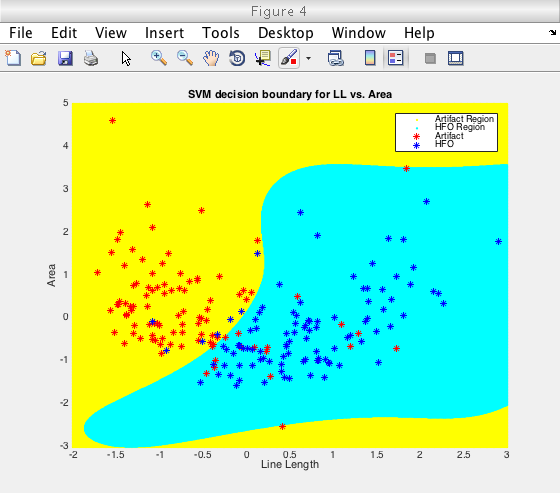
\includegraphics [width=4in]{mlautman_hw4_04.eps}

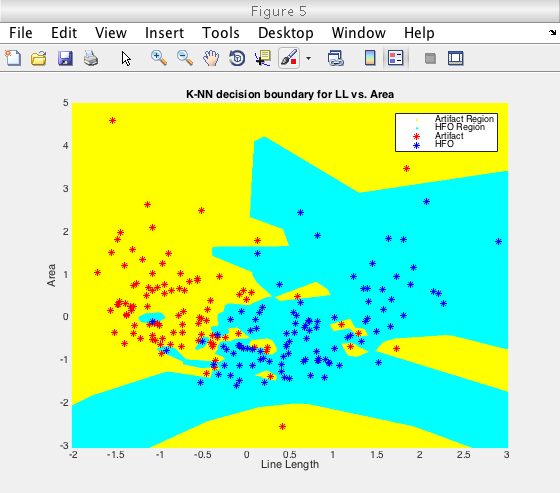
\includegraphics [width=4in]{mlautman_hw4_05.eps}

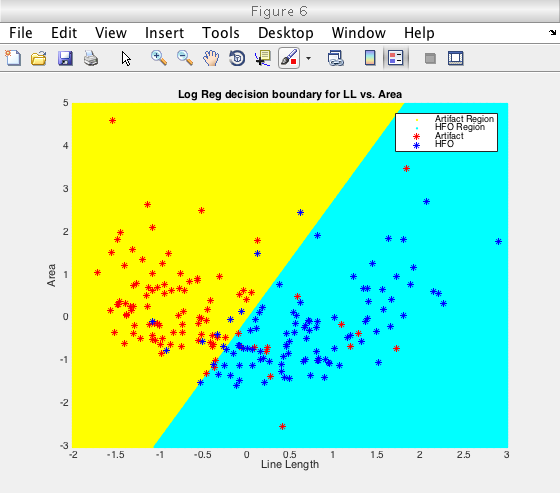
\includegraphics [width=4in]{mlautman_hw4_06.eps}
\begin{par}

\subsection*{3.6 Observations}
K-NN has clearly overfit the data by the furthest while logistic
regression has underfit the data by the furthest. We also see that K-NN
has the most jagged decision boundary whilest SVM has a very curvatious
boundary.

\end{par} \vspace{1em}
\begin{par}

\section*{4 Cross-Validation}'

\end{par} \vspace{1em}
\begin{par}

\subsection*{4.1 10 unique folds}'

\end{par} \vspace{1em}
\begin{verbatim}
clear folds
indices = randperm(length(trainFeats(:,1)));
folds{10} = trainFeats(1);
for i = 1:10
    s = max(1,round(length(indices)/10 * (i-1) + 1));
    e = min(length(indices), round(length(indices)/10 * i));
    folds{i} = indices(s:e)';
end

length(unique([folds{:}]))
\end{verbatim}

        \color{lightgray} \begin{verbatim}
ans =

   200

\end{verbatim} \color{black}
    \begin{par}

\subsection*{4.2.a Validation Error}'

\end{par} \vspace{1em}
\begin{verbatim}
[n, d] = size(trainFeats);
fold_n = 10;
fold_len = n / fold_n;

train_folds = zeros(fold_len * (fold_n - 1), d);
train_fold_class = zeros(fold_len * (fold_n - 1), 1);
test_folds = zeros(fold_len, d);
test_fold_class = zeros(fold_len, 1);
incorrect_pred = 0;

for i = 1:fold_n
    f_cnt = 0;

    % generate test and train sets
    for j = 1:10

        s = fold_len * (j - 1) + 1;
        e = fold_len * j;

        if i == j

            test_folds(1:fold_len, 1:d) = trainFeats(folds{j}, 1:d);
            test_fold_class(1:fold_len) = train_classes(folds{j});

        else
            f_cnt = f_cnt + 1;

            fold_s = fold_len * (f_cnt - 1) + 1;
            fold_e = fold_len * f_cnt;

            train_folds(fold_s:fold_e, 1:d) = trainFeats(folds{j}, 1:d);
            train_fold_class(fold_s:fold_e) = train_classes(folds{j});
        end
    end

    % run learning algorithms
    knn_pred_test = knnclassify(test_folds, train_folds, train_fold_class);
    incorrect_pred = incorrect_pred + sum(knn_pred_test ~= test_fold_class);

end
validation_error = incorrect_pred / n
\end{verbatim}

        \color{lightgray} \begin{verbatim}
validation_error =

    0.1950

\end{verbatim} \color{black}
    \begin{par}

\subsection*{4.2b}'
The error is higher. Since the training set leaves out the testing fold,
when we go to fit the testing fold to the model, we are matching up
points to the nearest neighbor wheras before we were matching those
points to themselves. Ultimately, we are avoiding testing on data that we
trained on so we would expect a higher error rate.

\end{par} \vspace{1em}
\begin{par}

\subsection*{4.3a validation error }'

\end{par} \vspace{1em}
\begin{verbatim}
knn_train_error = zeros(1,30);
validation_error = zeros(1,30);

for k = 1:30
    train_folds = zeros(fold_len * (fold_n - 1), d);
    train_fold_class = zeros(fold_len * (fold_n - 1), 1);

    test_folds = zeros(fold_len, d);
    test_fold_class = zeros(fold_len, 1);
    incorrect_pred = 0;

    for i = 1:fold_n
        f_cnt = 0;

        % generate test and train sets
        for j = 1:fold_n

            s = fold_len * (j - 1) + 1;
            e = fold_len * j;

            if i == j

                test_folds(1:fold_len, 1:d) = trainFeats(folds{j}, 1:d);
                test_fold_class(1:fold_len) = train_classes(folds{j});

            else
                f_cnt = f_cnt + 1;

                fold_s = fold_len * (f_cnt - 1) + 1;
                fold_e = fold_len * f_cnt;

                train_folds(fold_s:fold_e, 1:d) = trainFeats(folds{j}, 1:d);
                train_fold_class(fold_s:fold_e) = train_classes(folds{j});
            end
        end

        % run learning algorithms
        knn_pred_test = knnclassify(test_folds, train_folds, train_fold_class, k);

        incorrect_pred = incorrect_pred + sum(knn_pred_test ~= test_fold_class);

    end

    knn_pred_train = knnclassify(trainFeats, trainFeats, train_classes, k);
    knn_train_error(k) = sum(train_classes ~= knn_pred_train')/length(train_classes);
    validation_error(k) = incorrect_pred / (fold_len * fold_n);

end

figure(7)
hold on
plot(1:30, validation_error, 'b-o');
plot(1:30, knn_train_error, 'r-o');
title('Validation and training error for k-NN')
xlabel('k')
ylabel('error')
legend('validation error', 'training error')
\end{verbatim}

\includegraphics [width=4in]{mlautman_hw4_07.eps}
\begin{par}

\subsection*{4.3b optimal k}'

\end{par} \vspace{1em}
\begin{verbatim}
[lowest_error, best_k] = min(validation_error)
\end{verbatim}

        \color{lightgray} \begin{verbatim}
lowest_error =

    0.1150


best_k =

    10

\end{verbatim} \color{black}
    \begin{par}

\subsection*{4.3c overfitting with large k's}
If k gets large k-nn overfits less because for any given point, the
influence it has on a prediction goes down to 1/k. Increasing k
effectively smooths over the decision surface.

\end{par} \vspace{1em}
\begin{par}

\subsection*{4.4.a learning with an optimal k}

\end{par} \vspace{1em}
\begin{verbatim}
knn_pred_test = knnclassify(testFeats,trainFeats, train_classes, best_k);
knn_test_error = sum(knn_pred_test' ~= test_classes)/length(test_classes)
\end{verbatim}

        \color{lightgray} \begin{verbatim}
knn_test_error =

    0.1310

\end{verbatim} \color{black}
    \begin{par}

\subsection*{4.4.a learning with an optimal k}
The cross-validated model's testing error is less than the error from the
model trained in question 3.3. The best model from question 3.3 used
support vectors.

\end{par} \vspace{1em}



\end{document}
    
